\section{1174050 Dika Sukma Pradana}
\subsection{Teori}
\begin{enumerate}
\item Kenapa file suara harus di lakukan MFCC. dilengkapi dengan ilustrasi atau gambar. \\
\par Nilai-nilai MFCC meniru pendengaran manusia dan mereka biasanya digunakan dalam aplikasi pengenalan suara serta genre musik
deteksi. Nilai-nilai MFCC ini akan dimasukkan langsung ke jaringan saraf.Agar dapat diubah menjadi bentuk vektor, dan dapat digunakan pada machine learning. Disebabkan machine learning hanya mengerti bilangan vektor saja.\\
\begin{figure}[ht]
\centering
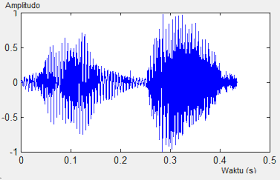
\includegraphics[scale=0.5]{figures/1174050/chapter6/7.png}
\caption{Contoh MFCC}
\label{Teori}
\end{figure}
Ilustrasinya, Ketika ingin menggunakan file suara dalam machine learning, misalnya untuk melihat jam. Machine learning tidak memahami rekaman suara melainkan vektor. Maka rekaman tersebut akan diubah kedalam bentuk vektor kemudian vektor akan menyesuaikan dengan kata kata yang sudah disediakan. Jika cocok maka akan mengembalikan waktu yang diinginkan

\item Konsep dasar neural network dilengkapi dengan ilustrasi atau gambar
\par Neural Network ini terinspirasi dari jaringan saraf otak manusia. Dimana setiap neuron terhubung ke setiap neuron di lapisan berikutnya. Lapisan pertama menerima input dan lapisan terakhir memberikan keluaran. Struktur jaringan, yang berarti jumlah neuron dan koneksinya, diputuskan sebelumnya dan tidak dapat berubah, setidaknya tidak selama training. Juga, setiap input harus memiliki jumlah nilai yang sama. Ini berarti bahwa gambar, misalnya, mungkin perlu diubah ukurannya agar sesuai dengan jumlah neuron input.\\
\begin{figure}[ht]
\centering
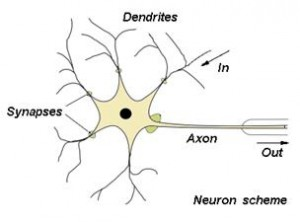
\includegraphics[scale=0.5]{figures/1174050/chapter6/8.jpg}
\caption{Contoh Pembobotan Neural Network}
\label{Teori}
\end{figure}


\item Konsep pembobotan dalam neural network.dilengkapi dengan ilustrasi atau gambar
\par Bobot mewakili kekuatan koneksi antar unit. Jika bobot dari node 1 ke node 2 memiliki besaran lebih besar, itu berarti bahwa neuron 1 memiliki pengaruh lebih besar terhadap neuron. 2. Bobot penting untuk nilai input. Bobot mendekati nol berarti mengubah input ini tidak akan mengubah output. Bobot negatif berarti meningkatkan input ini akan mengurangi output. Bobot menentukan seberapa besar pengaruh input terhadap output. Seperti contoh berikut :
\begin{figure}[ht]
\centering
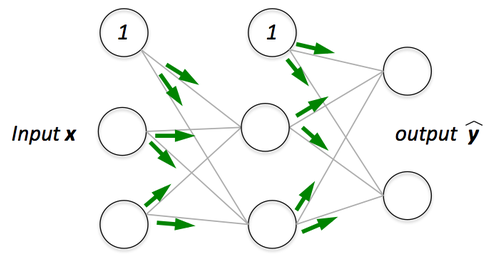
\includegraphics[scale=0.5]{figures/1174050/chapter6/2.png}
\caption{Contoh Pembobotan Neural Network}
\label{Teori}
\end{figure}

\item Konsep fungsi aktifasi dalam neural network. dilengkapi dengan ilustrasi atau gambar
\par Fungsi aktivasi digunakan untuk memperkenalkan non-linearitas ke jaringan saraf. Ini menekan nilai dalam rentang yang lebih kecil yaitu. fungsi aktivasi Sigmoid memeras nilai antara rentang 0 hingga 1. Ada banyak fungsi aktivasi yang digunakan dalam industri pembelajaran yang dalam dan ReLU, SeLU dan TanH lebih disukai daripada fungsi aktivasi sigmoid. Ilustrasinya, ketika fungsi aktivasi linier, jaringan saraf dua lapis mampu mendekati hampir semua fungsi. Namun, jika fungsi aktivasi identik dengan fungsi aktivasi F (X) = X), properti ini tidak puas, dan jika MLP menggunakan fungsi aktivasi yang sama, seluruh jaringan setara dengan jaringan saraf lapis tunggal.

\item Cara membaca hasil plot dari MFCC,dilengkapi dengan ilustrasi atau gambar\\
Berikut merupakan hasil plot dari rekaman suara :
\begin{figure}[ht]
\centering
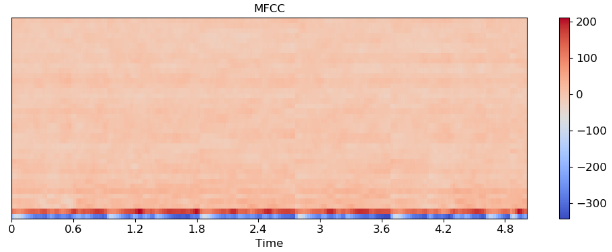
\includegraphics[scale=0.5]{figures/1174050/chapter6/1.png}
\caption{Cara Membaca Hasil Plot MFCC}
\label{Teori}
\end{figure}
Dari gambar tersebut dapat diketahui :\\
\begin{itemize}
\item Terdapat 2 dimensi yaitu x sebagai waktu, dan y sebagai power atau desibel.
\item Dapat dilihat bahwa jika berwarna biru maka power dari suara tersebut rendah, dan jika merah power dari suara tersebut tinggi
\item Dibagian atas terdapat warna merah pudar yang menandakan bahwa tidak ada suara sama sekali dalam jangkauan tersebut.
\end{itemize}

\item Jelaskan apa itu one-hot encoding,dilengkapi dengan ilustrasi kode dan atau gambar.
\par One-hot encoding adalah representasi variabel kategorikal sebagai vektor biner. Mengharuskan nilai kategorikal dipetakan ke nilai integer. Kemudian, setiap nilai integer direpresentasikan sebagai vektor biner yang semuanya bernilai nol kecuali indeks integer, yang ditandai dengan 1.
\begin{figure}[ht]
\centering
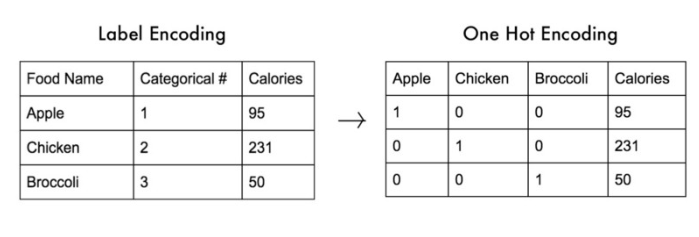
\includegraphics[scale=0.5]{figures/1174050/chapter6/3.png}
\caption{One Hot Encoding}
\label{Teori}
\end{figure}

\item fungsi dari np/.unique dan to categorical dalam kode program,dilengkapi dengan ilustrasi atau gambar.\\
Untuk np unique fungsinya yaitu menemukan elemen unik array. Mengembalikan elemen unik array yang diurutkan. Ada tiga output opsional selain elemen unik:\\
\begin{itemize}
\item Indeks array input yang memberikan nilai unik
\item Indeks array unik yang merekonstruksi array input
\item Berapa kali setiap nilai unik muncul dalam array input.
\end{itemize}
\begin{figure}[ht]
\centering
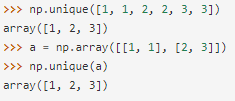
\includegraphics[scale=0.5]{figures/1174050/chapter6/4.png}
\caption{Numpy Unique}
\label{Teori}
\end{figure}

Untuk  To Categorical fungsinya untuk mengubah vektor kelas (integer) ke matriks kelas biner.
\begin{figure}[ht]
\centering
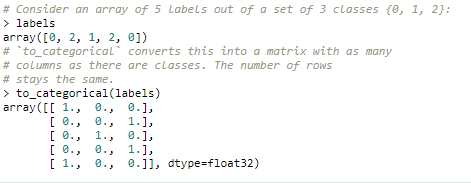
\includegraphics[scale=0.5]{figures/1174050/chapter6/5.png}
\caption{To Categorical}
\label{Teori}
\end{figure}

\item Fungsi dari Sequential dalam kode program,dilengkapi dengan ilustrasi atau gambar.\\
Sequential berfungsi sebagai tumpukan linear lapisan. COntohnya sebagai berikut :
\begin{figure}[ht]
\centering
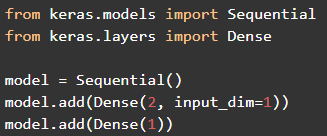
\includegraphics[scale=0.5]{figures/1174050/chapter6/6.png}
\caption{Sequential}
\label{Teori}
\end{figure}
\end{enumerate}


\subsection{Praktek}
\begin{enumerate}

\item Penjelasan isi data GTZAN Genre Collection dan data dari Freesound.
Isi data data merupakan datasets lagu atau suara yang terdiri dari 10 genre yang di simpan kedalam 10 folder yaitu folder blues, classical, country, disco, hiphop, jazz, metal, pop, reggae, dan rock ke sepuluh folder. Masing - masing dari folder terdapat 100 data suara sedangkan data freesound merupakan contoh data suara yang akan di gunakan untuk menguji hasil pengolahan data tersebut dengan menggunakan metode mfcc.
Code Yang Digunakan :
\lstinputlisting{src/1174050/chapter6/1.py}

\item Penjelasan perbaris kode program dari display MFCC.
\begin{itemize}
\item Code Yang Digunakan :
\lstinputlisting{src/1174050/chapter6/2.py}

\item Penjelasan:

\begin{enumerate}
\item Baris Code 1: Membuat fungsi display MFCC untuk menampilkan vektorisasi dari sebuah suara dimana variabel parameter.
\item Baris Code 2: Membuat variabel Y dimana untuk membaca variable parameter song dari perintah librosa load.
\item Baris Code 3: Membuat variabel MFCC untuk memanggil variabel Y dan mengubah suara menjadi vektor.
\item Baris Code 4: Melakukan plotting gambar dengan ukuran 10x4 dari figsize.
\item Baris Code 5: Menampilkan spektogram dari library librosa dimana untuk x\_axis didefinisikan dengan time kemudian y\_axis di definisikan dengan mel.
\item Baris Code 6: Menambahkan colorbar pada plot yang dijalankan.
\item Baris Code 7: Menetapkan atau memberikan judul untuk suara yang dieksekusi.
\item Baris Code 8: Untuk menyesuaikan subplot params sehingga subplot cocok dengan area gambar.
\item Baris Code 9: Fungsi untuk menampilkan hasil plot dari inputan yang telah dieksekusi.
\end{enumerate}

\item Ilustrasi Gambar:

\begin{figure}[!hbtp]
\centering
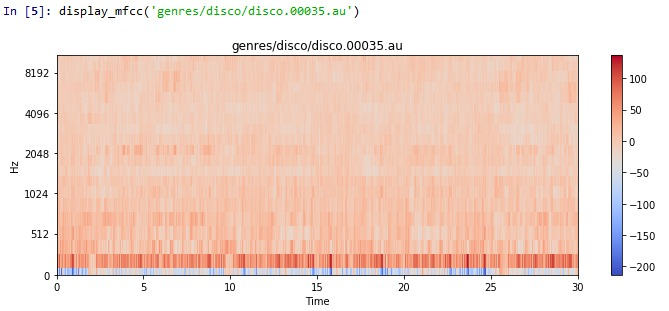
\includegraphics[scale=0.6]{figures/1174050/chapter6/11.jpeg}
\caption{Display MFCC}
\end{figure}

\end{itemize}

\item Penjelasan perbaris code dari Extract Feature Song.
\begin{itemize}
\item Code yang digunakan:
\lstinputlisting{src/1174050/chapter6/3.py}

\item Penjelasan Code:
\begin{enumerate}
\item Baris Code 1 : Membuat fungsi extract feature song dengan inputan parameter f
\item Baris Code 2 : Membuat variabel y dimana untuk meload atau membaca inputan parameter f dari perintah librosa load song 
\item Baris Code 3 : Membuat variabel mfcc yang difungsikan untuk membuat feature dari variabel y berdasarkan library librosa
\item Baris Code 4 : Membuat normalisasi nilai antara -1 sampai 1 yang didapatkan dari eksekusi np.absolute
\item Baris Code 5 : Didefinisikan untuk mengambil 25000 data pertama berdasarkan durasi suara atau musik lalu dikembalikan salinan arraynya dan dikecilkan menjadi satu.
\end{enumerate}

\item Ilustrasi Gambar:

\begin{figure}[!hbtp]
\centering
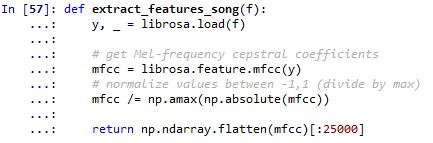
\includegraphics[scale=0.6]{figures/1174050/chapter6/12.jpg}
\caption{Extract Features Song}
\end{figure}

\item Mengapa yang diambil merupakan 25.000 baris data pertama?

Biar supaya tidak terjadi overhead pada komputer atau laptop atau proses eksekusi tidak terlalu lama.

\end{itemize}

\item Penjelasan perbaris code dari Generate Features and Labels.
\begin{itemize}

Code yang digunakan:
\lstinputlisting{src/1174050/chapter6/4.py}

\item Penjelasan:
\begin{enumerate}
\item Baris Code 1: Membuat perintah untuk fungsi generate features and labels.
\item Baris Code 2: Pembuatan variabel all features dengan array atau parameter kosong.
\item Baris Code 3: Pembuatan variabel all labels dengan array atau parameter kosong.
\item Baris Code 4: Mendefinisikan variable genres yang didalamnya berisi nama folder-folder pada variabel genres tersebut.
\item Baris Code 5: Membuat perintah fungsi looping.
\item Baris Code 6: Membuat atribut sound files yang berisi perintah looping perfolder dari folder genres dan mengambil semua file berekstensi au.
\item Baris Code 7: Memunculkan jumlah song yang dieksekusi.
\item Baris Code 8: Membuat perintah fungsi dari sound files.
\item Baris Code 9: Membuat variabel features untuk memanggil fungsi extract features song (f) sebagai inputan. Setiap satu file array sound files dilakukan ekstrak fitur.
\item Baris Code 10: Memasukkan semua features menggunakan perintah append kedalam all features.
\item Baris Code 11: Memasukkan semua genres menggunakan perintah append ke dalam all labels.
\item Baris Code 12:Mendefinisikan label uniq ids dan label row ids sebagai variabel dimana mengeksekusi perintah np.unique dengan parameter variabelnya all labels dan return inverse=True.
\item Baris Code 13: Membuat variabel label row ids untuk menentukan type dari variabel tersebut dengan type bit yang sesuai dengan yang digunakan.
\item Baris Code 14: Membuat variabel onehot labels dimana mengeksekusi to categorical dengan variabel parameter low row ids dan len.
\item Baris Code 15: Mengembalikan dan menampilkan hasil eksekusi dari variabel parameter all features dan onehot labels perintah dari np.stack.
\end{enumerate}

\item Ilustrasi Gambar:

\begin{figure}[!hbtp]
\centering
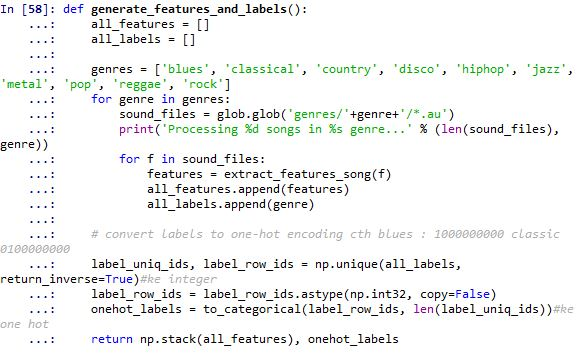
\includegraphics[scale=0.6]{figures/1174050/chapter6/13.jpg}
\caption{Generate Features and Label}
\end{figure}

\end{itemize}

\item Penjelasan penggunaan fungsi Generate Features and Labels sangat lama ketika Meload Dataset Genre.
\begin{itemize}

\item Code yang digunakan:
\lstinputlisting{src/1174050/chapter6/5.py}

\item Penjelasan:

Baris 1: Variabel features and label akn mengeksekusi isi dari features and label

Baris 2: Memproses 100 lagu di genre blues

Baris 3: Memproses 100 lagu di  genre classical

Baris 4: Memproses 100 lagu di  genre country

Baris 5: Memproses 100 lagu di  genre disco

Baris 6: Memproses 100 lagu di  genre  hip hop

Baris 7: Memproses 100 lagu di  genre jazz

Baris 8: Memproses 100 lagu di  genre metal

Baris 9: Memproses 100 lagu di genre pop

Baris 10: Memproses 100 lagu di genre reggae

Baris 11: Memproses 100 lagu di genre rock

\item Ilustrasi Gambar:

\begin{figure}[!hbtp]
\centering
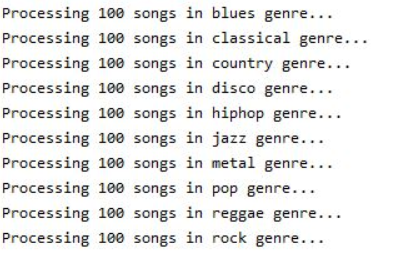
\includegraphics[scale=0.7]{figures/1174050/chapter6/18.PNG}
\caption{Fungsi Generate Features and Label Load Dataset Genre}
\end{figure}

\end{itemize}

\item Kenapa harus dilakukan pemisahan data training dan dataset sebesar 80\%

Code Yang Digunakan :
\lstinputlisting{src/1174050/chapter6/6.py}

\begin{itemize}
\item Penjelasan:

Untuk kemudahan dalam melakukan pengacakan, sebesar 80\% untuk data training dan 20\% untuk data test. Sehingga memperlihatkan bahwa data dipisah dan dipecah berpatokan dengan ketentuan 80\%. Untuk hasil pertama data trainingnya ada 800 baris dengan 25000 kolom dan data set sebanyak 200 baris dengan 10 kolom, sedangkan untuk hasil kedua yang telah digabungkan dengan one-hot encoding maka data training terdapat 800 baris dan data set dengan 200 baris namun keduanya memiliki jumlah kolom yang sama yaitu 25010.

\item Ilustrasi Gambar:

\begin{figure}[!hbtp]
\centering
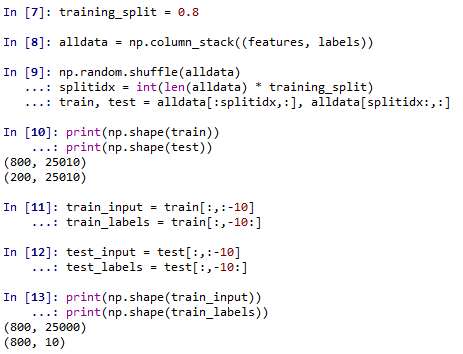
\includegraphics[scale=0.7]{figures/1174050/chapter6/19.png}
\caption{Pemisahan Data Training dan Dataset}
\end{figure}

\end{itemize}

\item Parameter dari fungsi Sequensial()

Code Yang Digunakan :
\lstinputlisting{src/1174050/chapter6/7.py}

\begin{itemize}
\item Penjelasan:

Untuk layer pertama densenya dari 100 neuron kemudian untuk inputan activationnya menggunakan fungsi relu. Dense 10 mengkategorikan 10 neuron untuk jenis genrenya untuk keluarnnya menggunakan aktivasi yaitu fungsi Softmax.

\item Ilustrasi Gambar:

\begin{figure}[!hbtp]
\centering
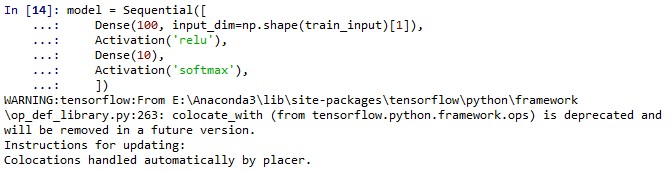
\includegraphics[scale=0.7]{figures/1174050/chapter6/20.png}
\caption{Parameter Fungsi Sequensial}
\end{figure}

\end{itemize}

\item Parameter dari fungsi Compile().

Code Yang Digunakan :
\lstinputlisting{src/1174050/chapter6/8.py}

\begin{itemize}
\item Penjelasan:

Untuk dilakukan pemrosesan menggunakan algortima adam sebagai optimizer yang sudah didefinisikan. Kemudian adam tersebut merupakan algoritma pengoptimalan dan untuk memperbarui bobot jaringan yang berulang berdasarkan data training sebelumnya. Untuk loss sendiri menggunakan categorical crossentropy yang difungsikan sebagai optimasi skor atau accuracy. Dan model tersebut digabungkan serta disimpulkan kemudian dicetak.

\item Ilustrasi Gambar:

\begin{figure}[!hbtp]
\centering
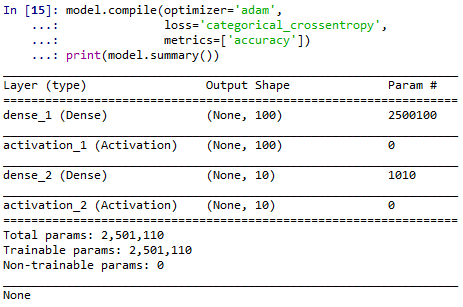
\includegraphics[scale=0.7]{figures/1174050/chapter6/21.png}
\caption{Parameter Fungsi Compile}
\end{figure}

\end{itemize}

\item Parameter dari fungsi Fit().

Code Yang Digunakan :
\lstinputlisting{src/1174050/chapter6/9.py}

\begin{itemize}
\item Penjelasan:

Untuk dilakukan pelatihan dengan epoch dengan rambatan balik sebanyak 10, kemudian dalam sekali epochs dilakukan 32  sampel yang diproses sebelum model diperbarui. Dilakukan validation split sebesar 20\% untuk melakukan pengecekan pada cross score validation yang telah dilakukan.

\item Ilustrasi Gambar:

\begin{figure}[!hbtp]
\centering
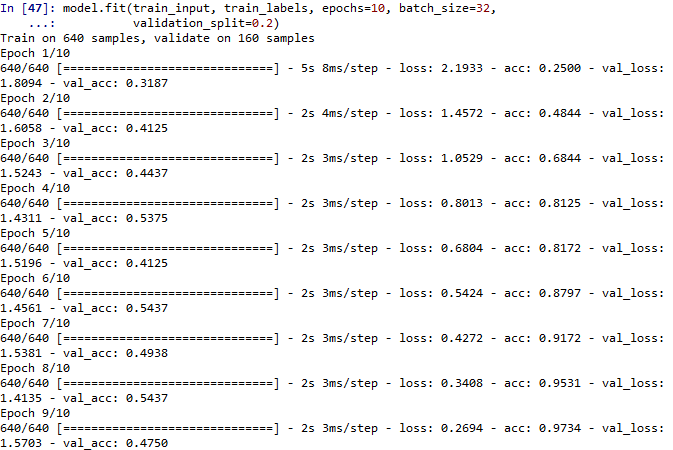
\includegraphics[scale=0.7]{figures/1174050/chapter6/22.png}
\caption{Parameter Fungsi Fit}
\end{figure}

\end{itemize}

\item Parameter dari fungsi Evaluate()

Code Yang Digunakan :
\lstinputlisting{src/1174050/chapter6/10.py}

\begin{itemize}
\item Penjelasan:

Untuk menggunakan test input dan test label dilakukan evaluasi atau proses menemukan model terbaik yang mewakili data dan seberapa baik model yang dipilih akan dijalankan kedepannya. Kemudian pada hasilnya sendiri dapat dilihat bahwa Loss merupaka hasil prediksi yang salah sebanyak 1,7985 dan keakurasian prediksinya sebesar 0,4200.

\item Ilustrasi Gambar:

\begin{figure}[!hbtp]
\centering
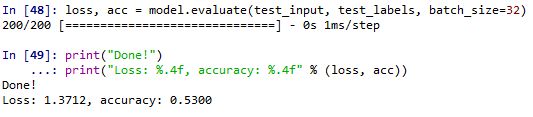
\includegraphics[scale=0.7]{figures/1174050/chapter6/23.png}
\caption{Parameter Fungsi Evaluate}
\end{figure}

\end{itemize}

\item Parameter dari fungsi Predict()

Code Yang Digunakan :
\lstinputlisting{src/1174050/chapter6/11.py}

\begin{itemize}
\item Penjelasan:

Untuk melakukan prediksi diambil dari satu baris berdasarkan test\_input . Nilai yang tertinggi terdapat pada label kedua yang dipilih prediksi yang tepat kemudian akan dikelompokkan.

\item Ilustrasi Gambar:

\begin{figure}[!hbtp]
\centering
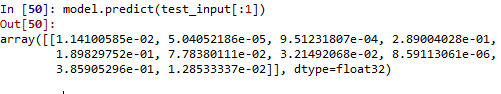
\includegraphics[scale=0.7]{figures/1174050/chapter6/24.png}
\caption{Parameter Fungsi Predict}
\end{figure}

\end{itemize}

\item PENANGANAN ERROR

\begin{itemize}

\item Ilustrasi Gambar:

\begin{figure}[!hbtp]
\centering
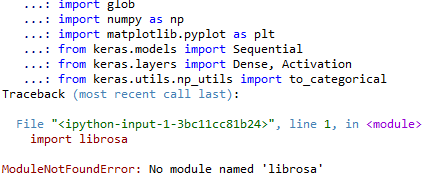
\includegraphics[scale=0.7]{figures/1174050/chapter6/error.png}
\caption{Error}
\end{figure}

\item Penjelasan:

 Install library tersebut pada Anaconda Prompt, jika proses penginstalan telah berhasil atau selesai dilakukan maka error akan teratasi.

\end{itemize}

\end{enumerate}